%=============================================================================
% ..... THIS IS chapter{Stereoop } .....
% 
% Revised Nov 2009: yusuke hiwasaki
%         May 2013: yusuke hiwasaki
%=============================================================================
\chapter{ITU-T Stereo processing tool}
%=============================================================================

\section{Introduction}

For the development and characterization of stereo algorithms,
properly conditioned stereo signals are required. To reuse the
existing set of STL single-channel processing tools for conditioning
the inputs and outputs in a stereo processing chain, a generic stereo
operations tool was developed and introduced in STL2009. This stereo
processing tool provides the basic functionalities of interleaving
single channel files, splitting stereo files into single channel
files, and creating specific single channel down-mix signals from a
given stereo input.
%\textcolor{blue}{In STL2014 release, this tool was revised to incorporate mid-side (MS) stereo conversion from a standard left-right (LR) format.}

\section{Description of the algorithm}

The tool operates on sample basis on 16-bit resolution input files,
and provides the following functionalities:

\begin{itemize}
\item Interleaving two single channel files into one single
  two-channel stereo file.
\item Splitting an interleaved two-channel file into individual single
  channel files 
\item Down-mixing a two-channel stereo file into a maximum channel
  energy analysis file (a single channel analysis signal for stereo
  scene level evaluation purposes).
\item Down-mixing a two-channel file into a single channel mono file
% $\item \textcolor{blue}{Converting a two-channel stereo file into two mid- and side-files, and reverse conversion from two MS files into a two-channel stereo file.
% This operation also can change the power of the files.}
\end{itemize}

Figure~\ref{fig:stereoopFig1} illustrates the functionality that
interleaves two single channel files into one single two-channel
stereo file. Figure~\ref{fig:stereoopFig2} illustrates the
functionality that splits an interleaved two-channel file into
individual single channel files. Figure~\ref{fig:stereoopFig3}
illustrates the functionality that down-mixes a two-channel file into
a maximum channel energy analysis file. Figure~\ref{fig:stereoopFig4}
illustrates the functionality that down-mixes a two-channel file into
a single channel mono
file.
% \textcolor{blue}{Figures~\ref{fig:stereoopFig5} and \ref{fig:stereoopFig6} illustrate the conversions between one single two-channel stereo file and a mid- and a side-channle files.}

\begin{figure}[htp]
    \begin{center}
        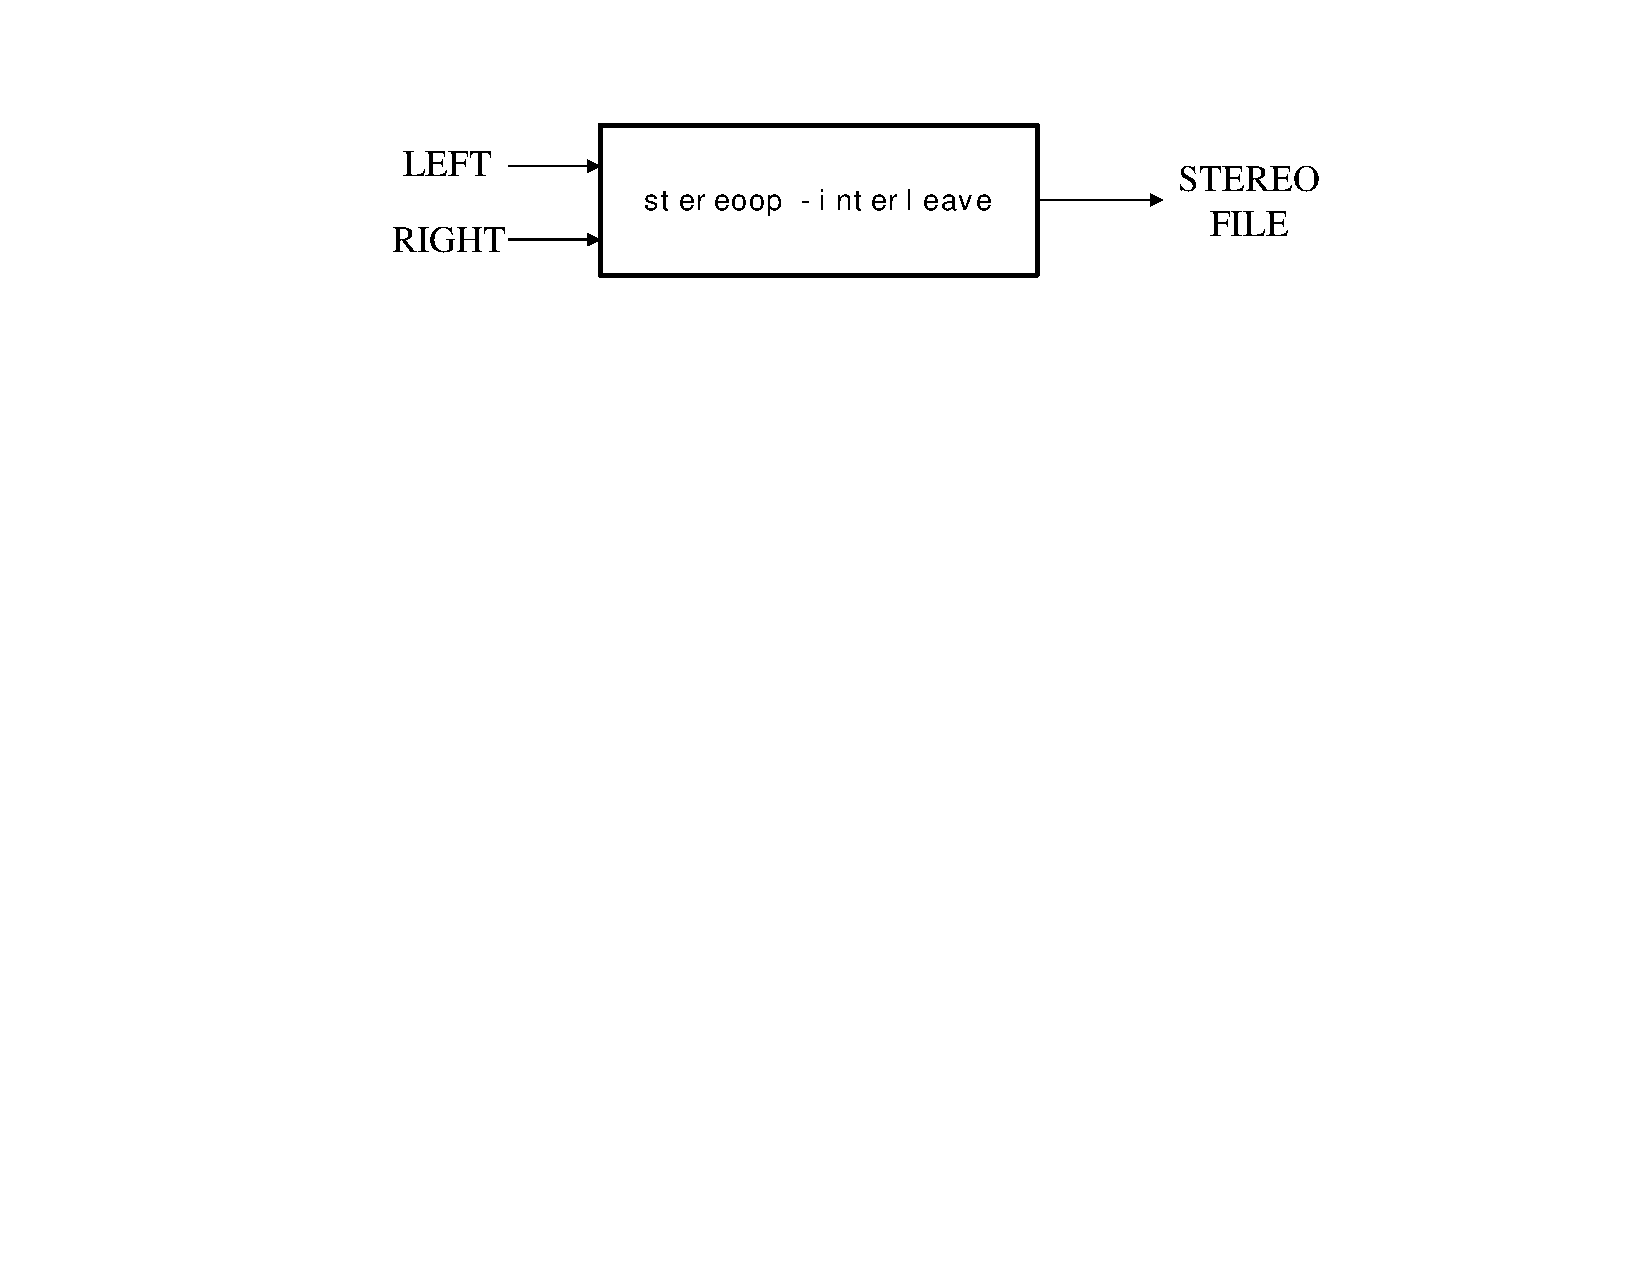
\includegraphics[scale=0.5]{stereoopFig1.pdf}
  \end{center}
  \caption{Interleaving two single channel files into one single two-channel stereo file.
           \label{fig:stereoopFig1} }
\end{figure}

\begin{figure}[htp]
    \begin{center}
        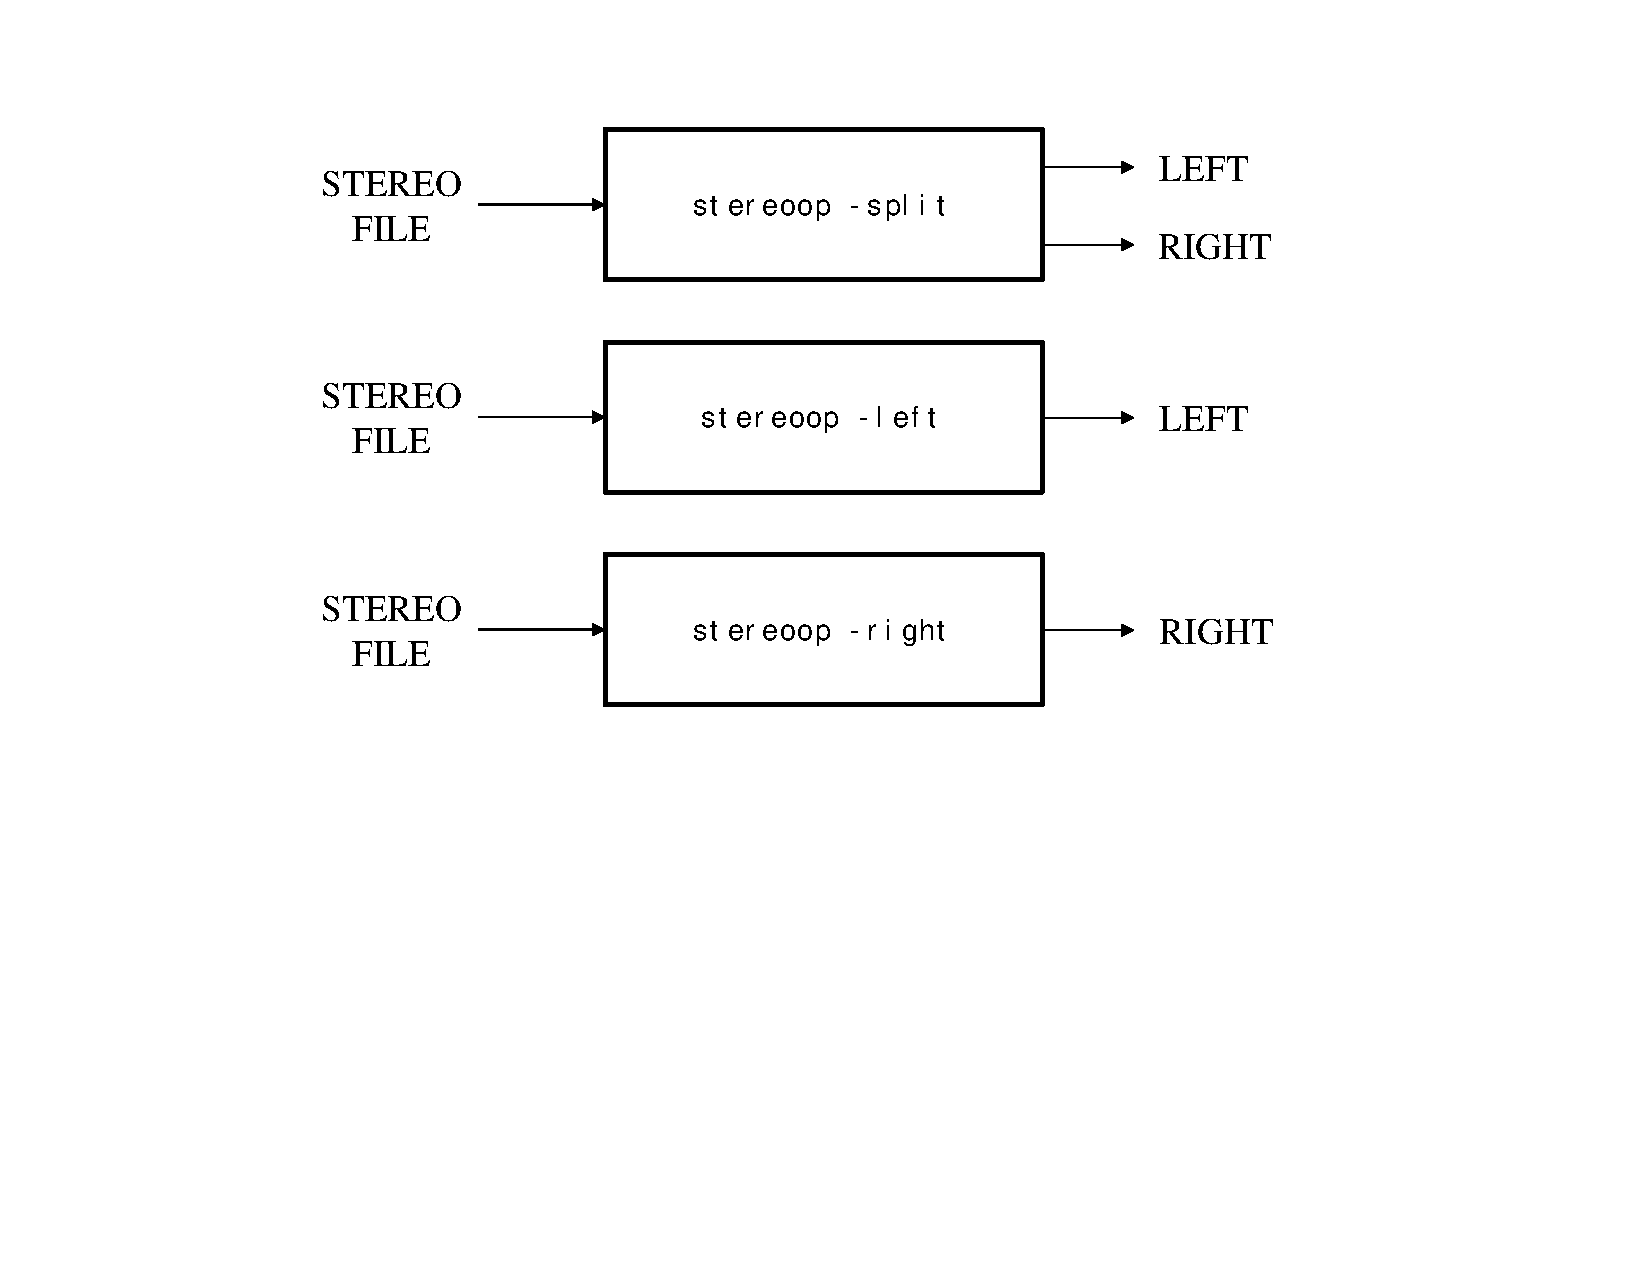
\includegraphics[scale=0.5]{stereoopFig2.pdf}
  \end{center}
  \caption{Splitting an interleaved two-channel file into two individual single channel files.
           \label{fig:stereoopFig2} }
\end{figure}

\begin{figure}[htp]
    \begin{center}
        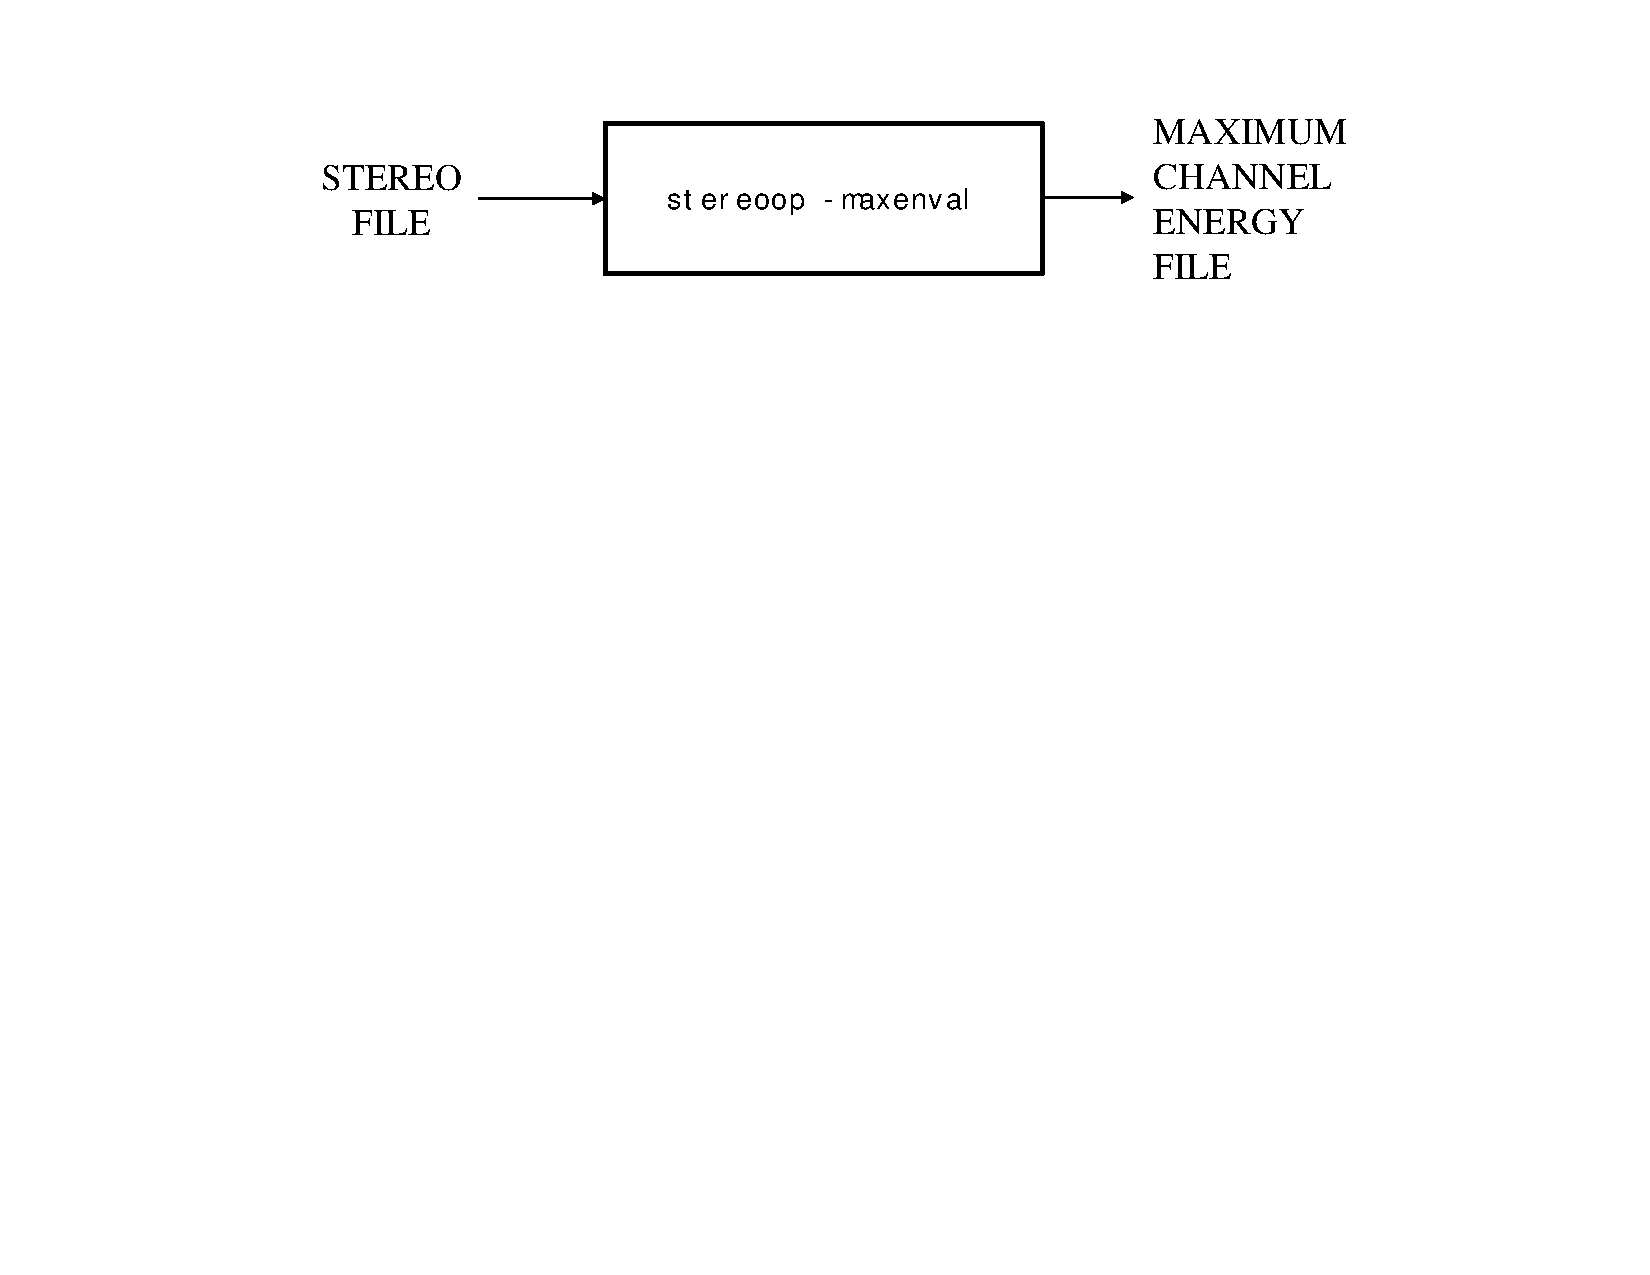
\includegraphics[scale=0.5]{stereoopFig3.pdf}
  \end{center}
  \caption{Down-mixing a two-channel file into a maximum channel energy analysis file.
           \label{fig:stereoopFig3} }
\end{figure}

\begin{figure}[htp]
    \begin{center}
        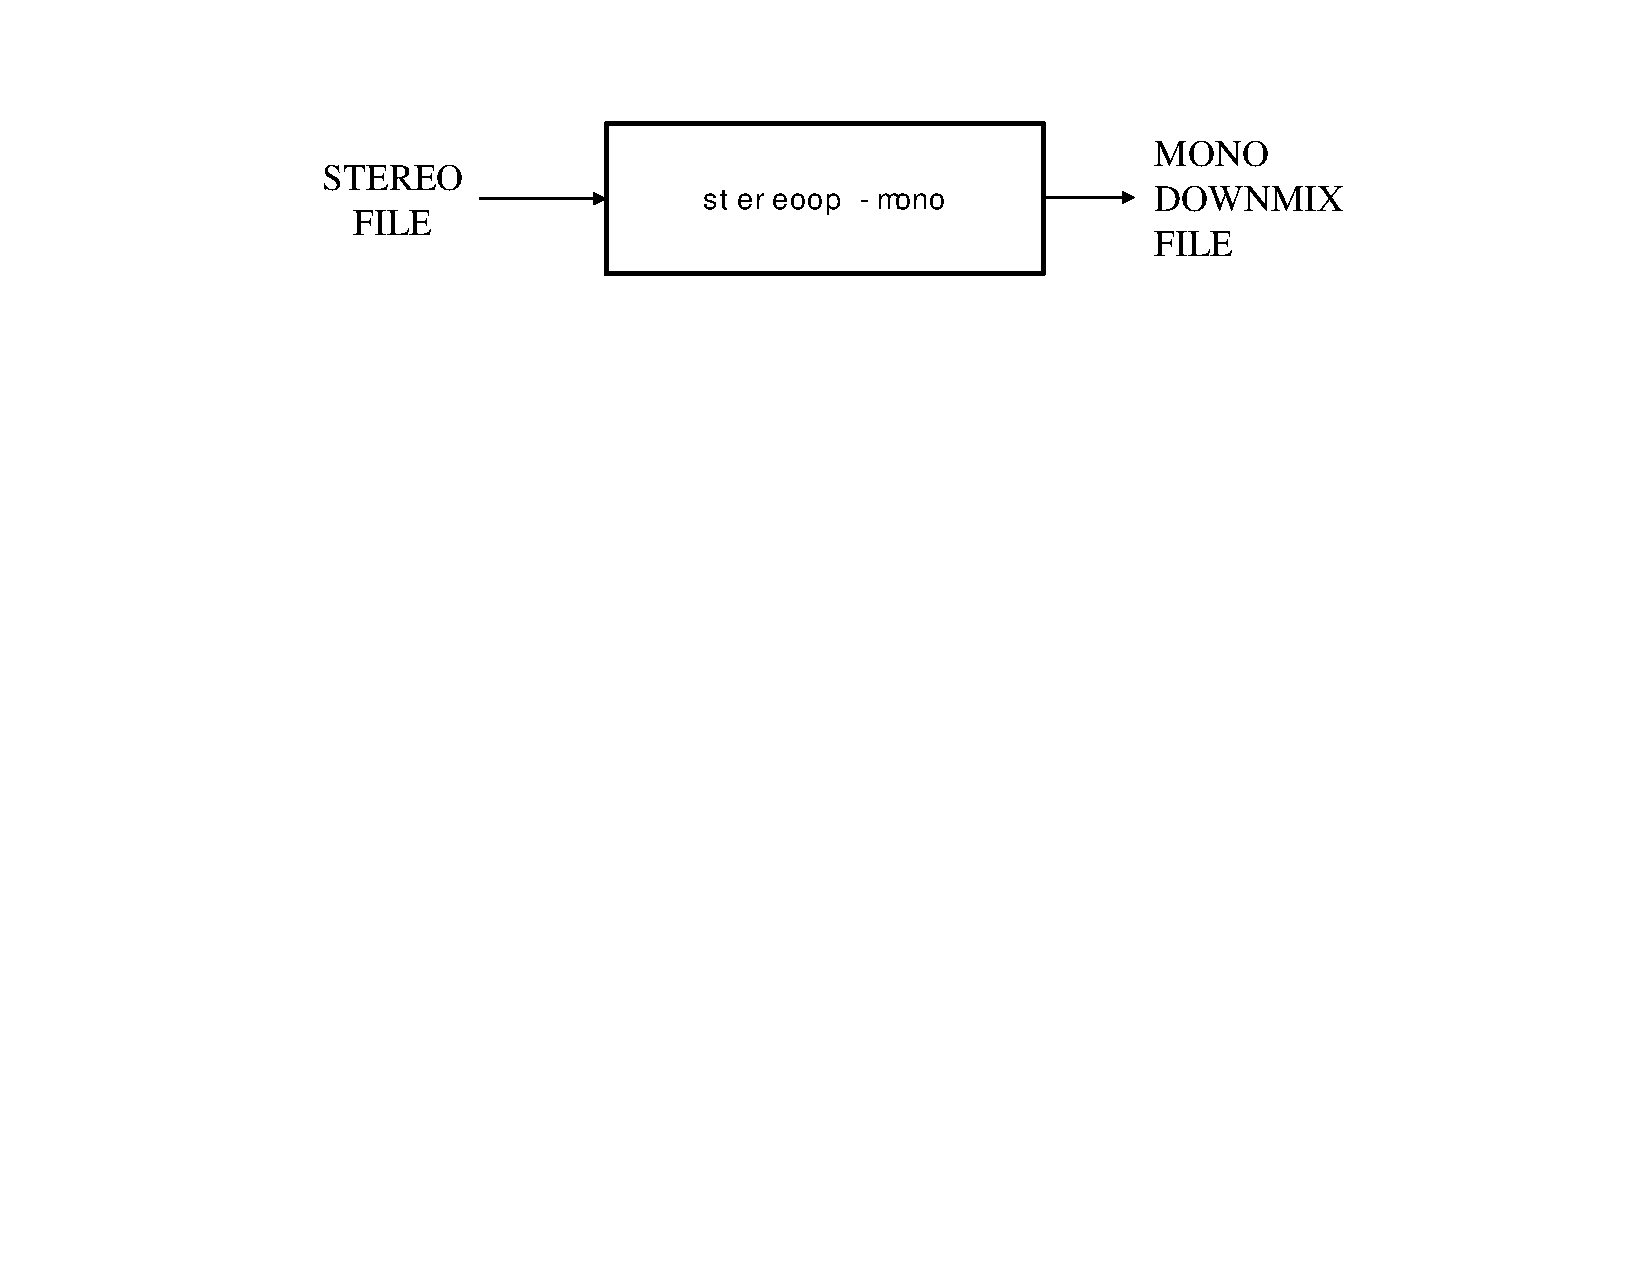
\includegraphics[scale=0.5]{stereoopFig4.pdf}
  \end{center}
  \caption{Down-mixing a two-channel file into a single channel mono file.
           \label{fig:stereoopFig4} }
\end{figure}

%\begin{figure}[htp]
%    \begin{center}
%        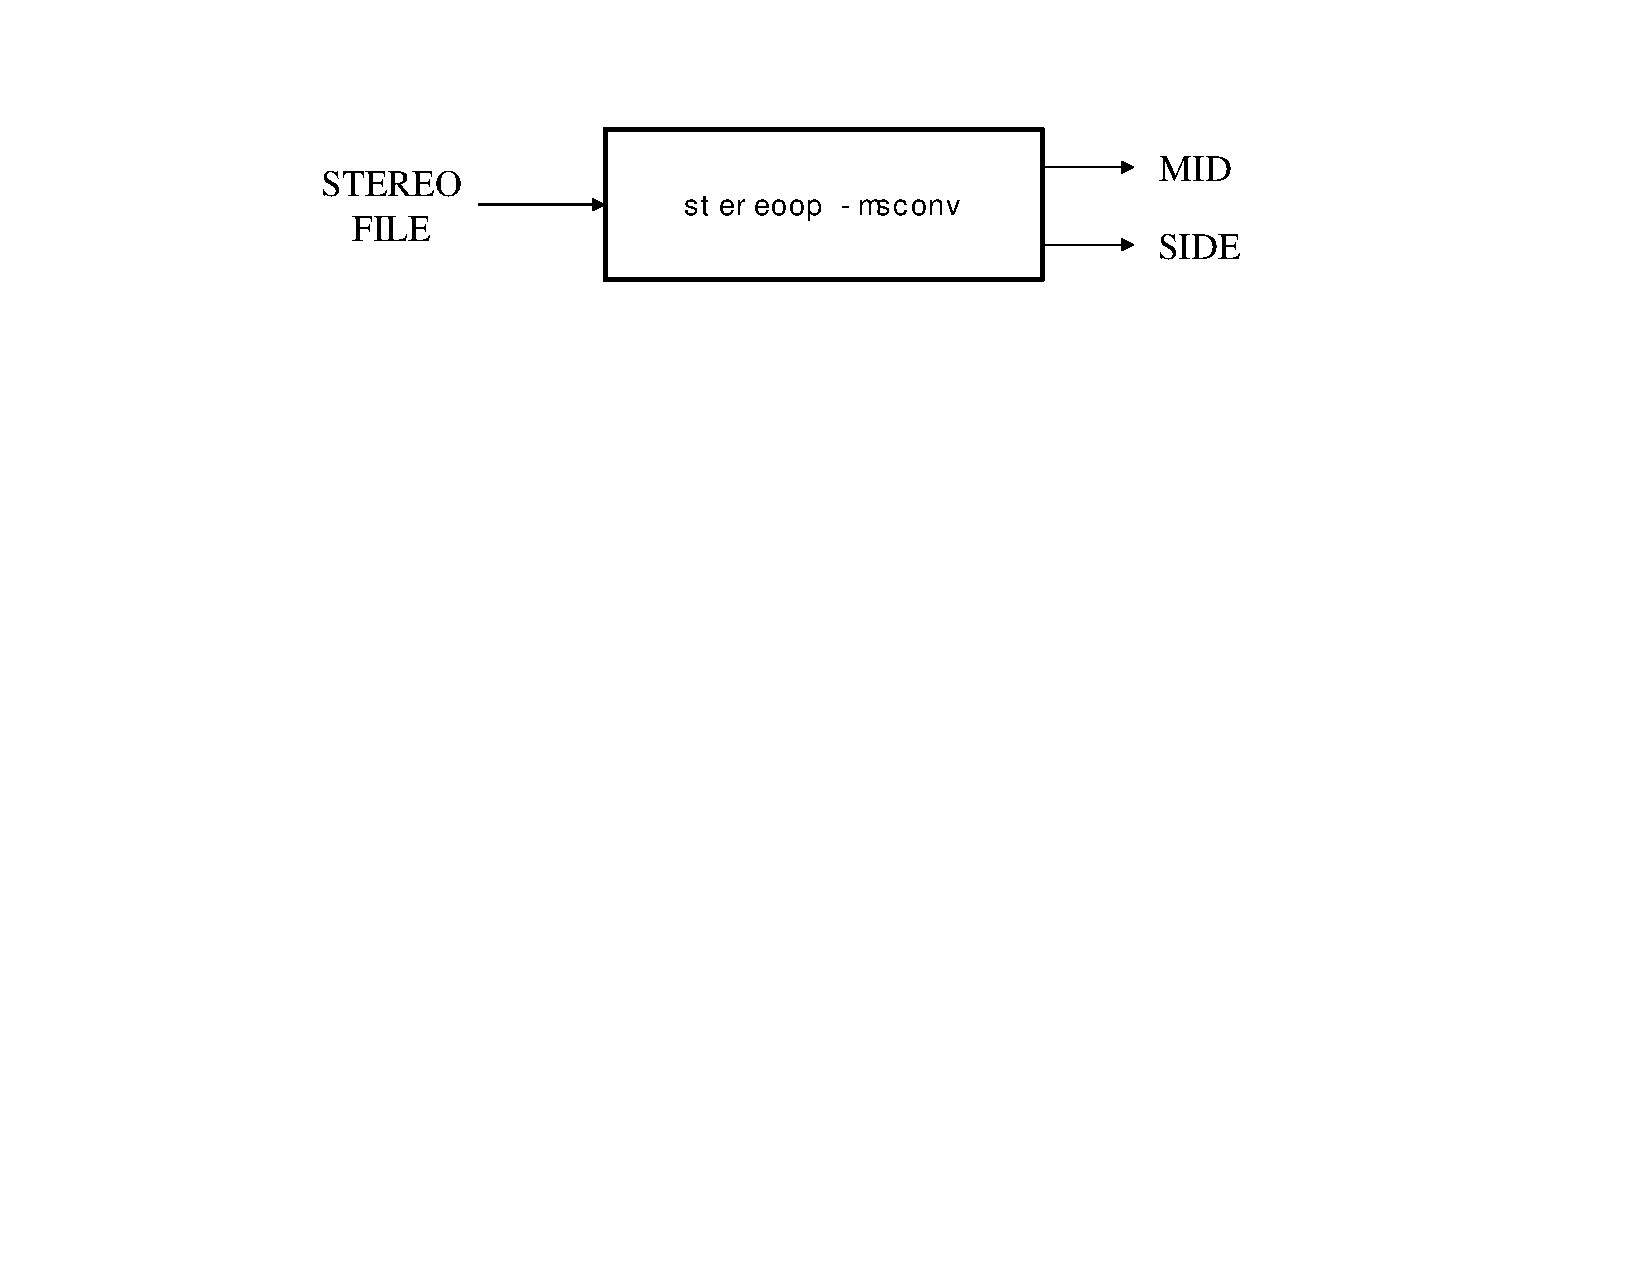
\includegraphics[scale=0.5]{stereoopFig5.pdf}
%  \end{center}
%  \caption{\textcolor{blue}{%
%      Converting a two-channel file into a mid- and a side-channel mono files.}
%           \label{fig:stereoopFig5} }
%\end{figure}

%\begin{figure}[htp]
%    \begin{center}
%        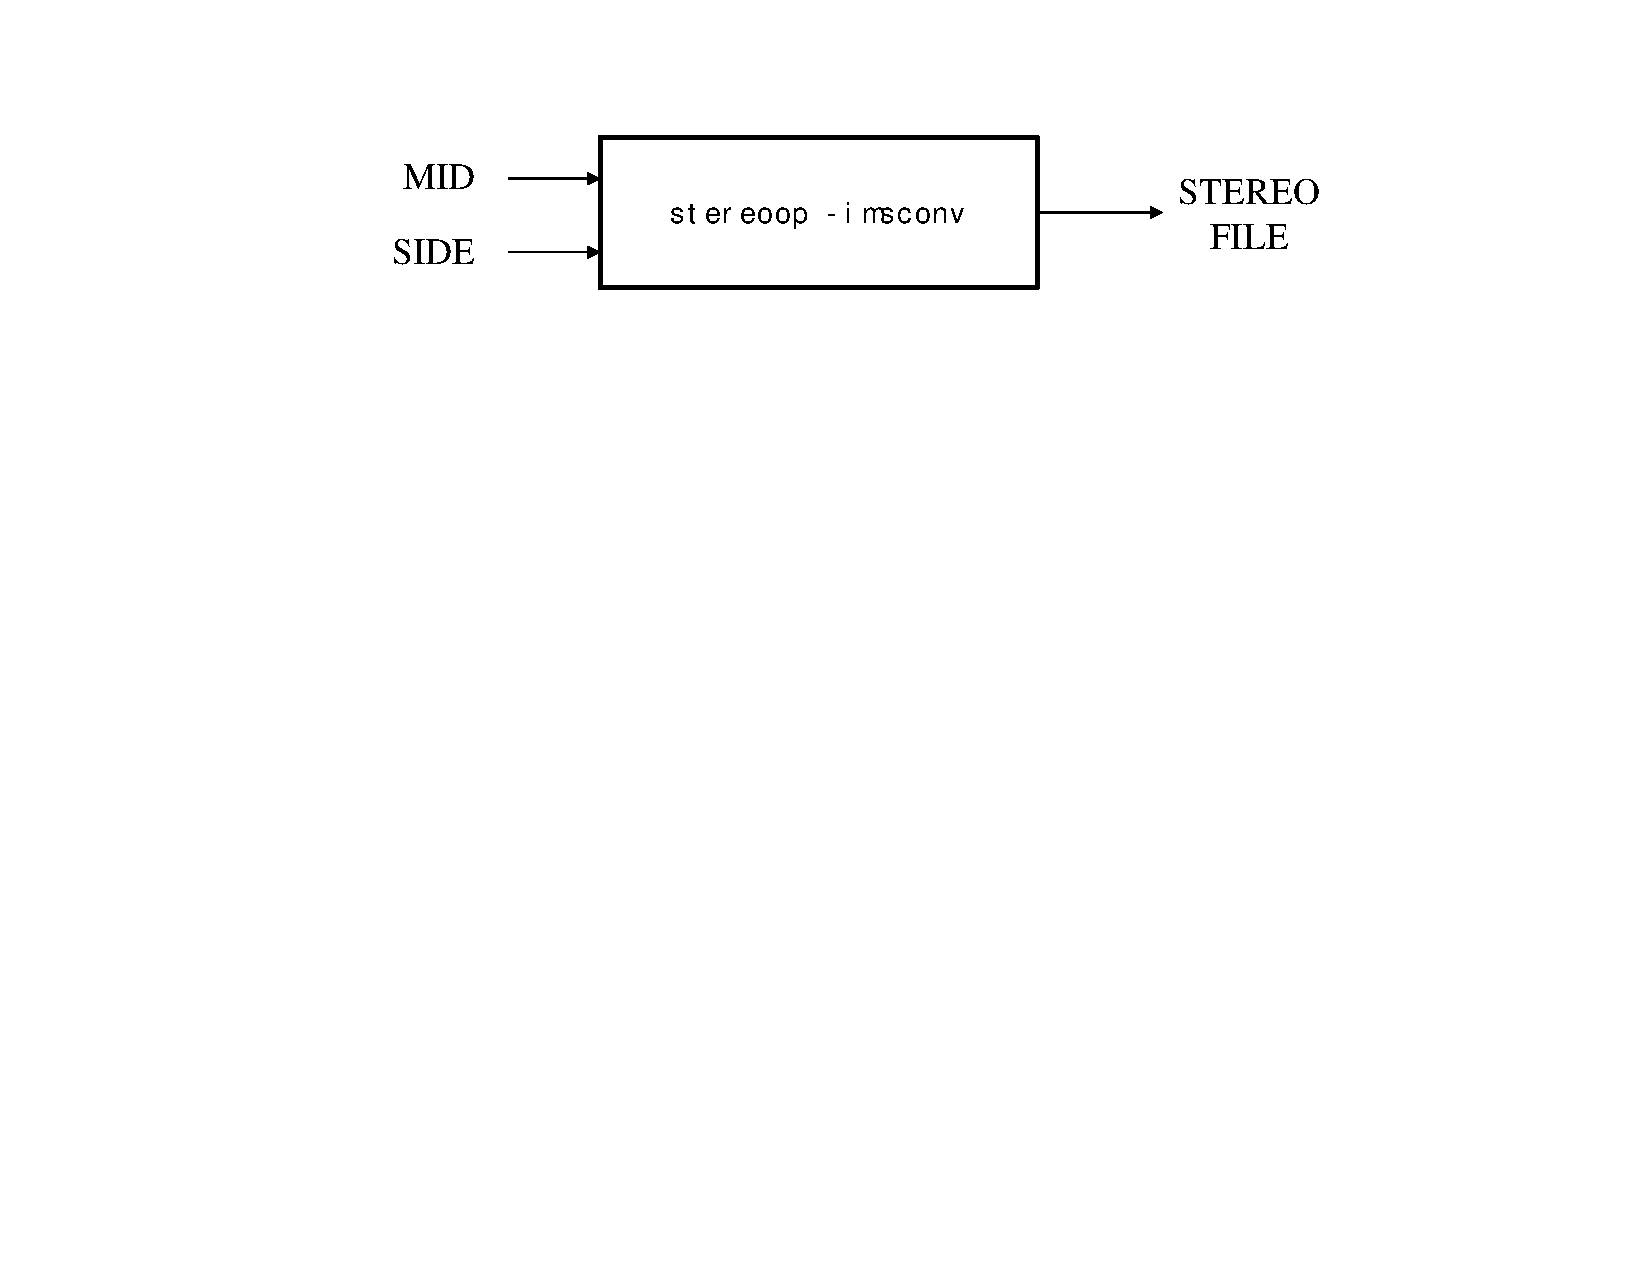
\includegraphics[scale=0.5]{stereoopFig6.pdf}
%  \end{center}
%  \caption{\textcolor{blue}{%
%      Converting a mid- and a side-channel files into a two-channel file.}
%           \label{fig:stereoopFig6} }
%\end{figure}

This set of stereo operation functionalities, in combination with the
existing STL tools which work on the single channel files, provides a
generic framework for stereo file processing.

\section{Implementation}

\subsection{Data and file format}
The tool works on 16-bit sample data (short), independent of sampling
frequency. It is assumed that left and right channels always have the
same sampling frequency.

File format: 2-channel data is stored in raw header-less files, with
each left channel sample stored before the corresponding right channel
sample. Single channel files are stored in raw header-less files as
required by most existing STL single channel tools.

The input and output file byte order will be the native system byte
order.

\subsection{stereoop module}

\subsubsection{Prototype}

{\tt {\small
\#include "ugstdemo.h"\\
enum Mode{ NONE = -1,INTER, SPLIT, LEFT, RIGHT, MAXENVAL, MONO,
%\textcolor{blue}{MSCONV, IMSCONV,}
N\_MODES };\\
int main (int argc, char *argv[]);
}}

\subsubsection{Description}

The main function opens the input file (or files) and processes them
according to a stereo operation option given on the command line and
stores the processed data into the output file (or files).

\subsubsection{Variables}

{\tt {\small
FILE   *Fif[MAX\_IFILES];	/* Pointer(s) to input files */ \\
FILE   *Fof[MAX\_OFILES];     	/* Pointer(s) to output files */ \\
char   ifname[MAX\_IFILES][MAX\_STR];	/* Input file names */ \\
char   ofname[MAX\_OFILES][MAX\_STR];	/* Output file names */ \\
enum   Mode mode=NONE; 	/* Operation mode variable */ \\
short  tmp\_short[2],tmp\_short\_1ch[1];	/* 16bit short read/write buffers */ \\
}}

\subsubsection{Command line syntax for channel manipulation operations}

{\tt {\small
\begin{tabular}{lllll}
stereoop & -interleave & infile.L.1ch      & infile.R.1ch  & outfile.stereo.2ch \\ 
stereoop & -split      & infile.stereo.2ch & outfile.L.1ch & outfile.R.1ch \\ 
stereoop & -left       & infile.stereo.2ch & outfile.L.1ch &  \\ 
stereoop & -right      & infile.stereo.2ch & outfile.R.1ch &  \\ 
\end{tabular} 
}}

\subsubsection{Command line syntax for channel down-mix operations}

{\tt {\small
\begin{tabular}{lllll}
stereoop & -maxenval & infile.stereo.2ch & outfile.maxenval.1ch  &  \\ 
stereoop & -mono     & infile.stereo.2ch & outfile.mono.1ch &  \\ 
\end{tabular} 
}}

%\textcolor{blue}{
%\subsubsection{Command line syntax for MS stereo operations}
%}
%\textcolor{blue}{
%{\tt {\small
%\begin{tabular}{llllll}
%stereoop & -msconv  & [-mult G] & infile.stereo.2ch & outfile.M.1ch & outfile.S.1ch \\
%stereoop & -imsconv & [-mult G] & infile.M.1ch & infile.S.1ch & outfile.stereo.2ch \\
%\end{tabular}
%}}
%}

\subsubsection{``stereoop -maxenval'' detailed operation}

The pseudo code below shows the tool operation when creating the
maximum channel energy downmix, a downmix that may be used for stereo
scene level evaluation purposes. The left or right sample value
yielding the maximum absolute value (which equals the value yielding
maximum energy) is written to the output file.

Pseudo code
{\tt\small
\begin{verbatim}
  [left, right] = ReadSamples(InputStereoChannelFile);

  if( |left| > |right|){
    output = left;
  } else {
    output = right;
  }
  WriteSample(OutputSingleChannelFile, output);
  }
\end{verbatim}}

\subsubsection{``stereoop -mono'' detailed operation}
The pseudo code below shows the tool operation when creating the mono
downmix. The output sample mono value is (left + right) / 2.0,
(rounded to a short value).

Pseudo code
{\tt\small
\begin{verbatim}
  [left, right] = ReadSamples(InputStereoChannelFile);

  output = ((double)left + (double)right)/2.0;

  WriteSample(OutputSingleChannelFile, round(output));
\end{verbatim}}

%\textcolor{blue}{
%\subsubsection{``stereoop -msconv'' detailed operation}
%The pseudo code below shows the tool operation when performing the LR-
%to MS-stereo conversion. The output mid- and side- sample mono value
%is (left + right) * Gain and (left - right) * Gain (both rounded to a
%short value), respectively. The default value of Gain is 0.5, unless
%specified with a {\tt -mult} option. It should be noted that due to
%the rounding, the LR-MS conversion may introduce some degradation.
%}
%
%\textcolor{blue}{
%Pseudo code
%}
%{\tt\small
%\begin{verbatim}
%  Gain = 0.5;
%
%  [left, right] = ReadSamples(InputStereoChannelFile);
%
%  m_output = ((double)left + (double)right) * Gain;
%  s_output = ((double)left - (double)right) * Gain;
%
%  WriteSample(OutputMChannelFile, round(m_output));
%  WriteSample(OutputSChannelFile, round(s_output));
%\end{verbatim}
%}
%
%\textcolor{blue}{
%\subsubsection{``stereoop -imsconv'' detailed operation}
%The pseudo code below shows the tool operation when performing the MS-
%to LR-stereo conversion. The output mid- and side- sample mono value
%is (left + right) * Gain and (left - right) * Gain (both rounded to a
%short value), respectively. The default value of Gain is 1.0, unless
%specified with a {\tt -mult} option. It should be noted that due to
%the rounding, the MS-LR conversion may introduce some degradation.
%}
%
%\textcolor{blue}{
%Pseudo code
%}
%{\tt\small
%\begin{verbatim}
%
%  Gain = 1.0;
%
%  mid_input  = ReadSamples(InputMChannelFile);
%  side_input = ReadSamples(InputSChannelFile);
%
%  left_output  = ((double)mid_input + (double)side_input) * Gain;
%  right_output = ((double)mid_input - (double)side_input) * Gain;
%
%  WriteSample(OutputStereoChannelFile, round([lef_output, right_output]);
%\end{verbatim}
%}

\section{Tests and Portability}
The stereoop tool example code has been evaluated under
Win2000/Cygwin(CYGWIN\_NT-5.0, v1.5.24/gcc(3.4.4), Linux
(2.6.5-7.145)/gcc(2.95.3) and Solaris(SunOS
Generic\_122300-02)/gcc(2.95.3).

\section{Example code}

A demonstration program, {\tt stereoop.c} implements the described
operations of the tool.
